%\section{GraphRNN: Generating Realistic Graphs with Deep Auto-Regressive Models}

\begin{center}
  \begin{tabular}{rl}
  % after \\: \hline or \cline{col1-col2} \cline{col3-col4} ...
  论文地址:& \href{https://arxiv.org/abs/1802.08773}{https://arxiv.org/abs/1802.08773} \\
  源码地址:& \href{https://github.com/snap-stanford/GraphRNN}{GraphRNN} \\
  关键词:& \textbf{RNN, Graph generation} \\
  写于:& \date{2020-09-18}
  \end{tabular}
\end{center}
% \par 论文地址:\href{https://arxiv.org/abs/1802.08773}{https://arxiv.org/abs/1802.08773}
% \par 源码地址:\href{https://github.com/snap-stanford/GraphRNN}{GraphRNN}
% \par 关键词:\textbf{RNN, Graph generation}
% \par 写于:\date{2020-09-18}

论文\cite{you2018graphrnn}提出了一个深度自回归(deep autoregressive)模型,用于图的生成。GraphRNN使用序列的生成概念对图的生产进行建模。为了定量地评估GraphRNN的性能,论文中使用MMD(Maximum Mean Discrepancy)的变体来衡量训练的图数据集和生成的图数据集之间的差异. 
\par 首先介绍图生成的应用。生产与真实图类似的图在很多领域都有重要的应用,例如对物理、社会进行建模,药物、分子结构的发现,构建知识图谱等。
现有的图生成的方法可以分为以下几种:\\
传统的图生成方法中,有Kronecker graphs, exponential random graphs, stocastic models等。传统的方法主要依靠手工构建特征,来生成指定特征的图,这种方法并不能直接在图数据(例如很多分子的图)中学习模型进而得到图生成模型。\\
近期也有一些深度生成模型被提出,如VAE(variational autoencoders), GAN(generative adversarial networks)\cite{kingma2014auto,goodfellow2014generative}。并且已经有一些基于深度生成模型的图生成方法,如\cite{simonovsky2018graphvae,li2018learning}。但是这些深度生成模型在生成图时依然存在一些不足,如只能从单一的图进行学习或者只能生成结点数较少的图(如少于40)。
\par 图生成问题中的几个难点:
\begin{itemize}
    \item 生成空间太大且可变。要制定具有n个结点的图需要$n^2$个值来确定边,并且结点和边的数量是不确定的。
    \item 表示不唯一。个人理解是因为图的同构性导致的。
    \item 复杂的依赖关系。边的生成并不是独立的,先后生成的边之间是存在依赖关系。\cite{li2018learning} 中提出了解决这个问题的方法,但是复杂度太高。
\end{itemize}

\par 接下来是GraphRNN 的细节。
首先先看看如何将一个图看作序列生成的过程。
对于一个给定的图$G$,图中共$n$个结点,下式中 $A^{\pi}_{ij}$ 为$G$的邻接矩阵,$\pi$ 为结点的某个排列。则$G$可以表示成如下形式: 
$$
S^\pi = (S^{\pi}_1,...,S^{\pi}_n)
$$
其中 $S^{\pi}_i = (A^{\pi}_{1,i},..., A^{\pi}_{i-1,i}), \forall i \in {2,...,n} $,其实就相当于邻接矩阵的第$i$列的上半部分,表示第$i$个结点与之前$i-1$个结点的连接关系。
Okay,图的序列表示解释到此为止。

\par 根据以上的解释,则一个图出现的概率$p(G)$可以表示为联合概率分布$p(G, S^{\pi})$ 关于$G$的边缘分布,令$S$表示$G$所有可能的排列,即
$$
p(G) = \sum_{S^{\pi} \in S } p(S^{\pi}) 
$$
对于某个排列$S^{\pi}$, $p(S^{\pi}) = \prod_{i=1}^{n+1} p(S^{\pi}_i | S^{\pi}_1,...,p^{\pi}_{i-1})$, 将$p(S^{\pi}_i | S^{\pi}_1,...,p^{\pi}_{i-1})$简化表示为$p(S^{\pi}_i | S^{\pi}_{<i})$。其实意义很明显,即当前结点的某条边的概率取决于该结点已经有的边情况。

\par 现在假设已经获得了生成模型,那么如何去生成一个图呢?过程如下。
\begin{algorithm}[H]
    \begin{algorithmic}[1]
        \textbf{Input}: RNN-based transition module $f_{trans}$, output\ module\ $f_{out}$, \newline
        probability\ distribution\ $\mathcal{P}_{\theta_{i}}$\ parameterized\ by\ $\theta_{i}$, start\ token\ SOS, end\ token\  EOS, empty\ graph\ state\ $h^{'}$ \newline
        \textbf{Output}: Graph\ sequence\ $S^{\pi}$
        $S^{\pi}_1=SOS, h_1=h^{'}, i=1$ \newline
        \textbf{repeat} \newline
            $i = i+1$ \newline
            $h_i = f_{trans}(h_{i-1}, S^{\pi}_{i-1})\{update\ graph\ state\}$\newline
            $\theta_i = f_{out}(h_i)$ \newline
            $S^{\pi}_{i} \sim \mathcal{P}_{\theta_i}\{smaple\ node\ i's\ edge\ connections\}$ \newline
        \textbf{until}\ $S^{\pi}_i$\ is\ EOS \newline
        \textbf{Return}\ $S^{\pi} = (S^{\pi}_1,...,S^{\pi}_i)$ \newline
    \end{algorithmic}
    \caption{GraphRNN inference algorithm }
\end{algorithm}

那么剩下的就是如何去获得上面算法中即生成模型的参数了。
GraphRNN使用深度学习的方法来建模图生成的问题,不需要人为的去构建特征来生成指定特征的图,能以图数据为基础来生成类似的图,重点在于如何设计GraphRNN的模型结构。
\par 如图1所示为GraphRNN生成图的过程。
\begin{figure}[h]
    \centering
    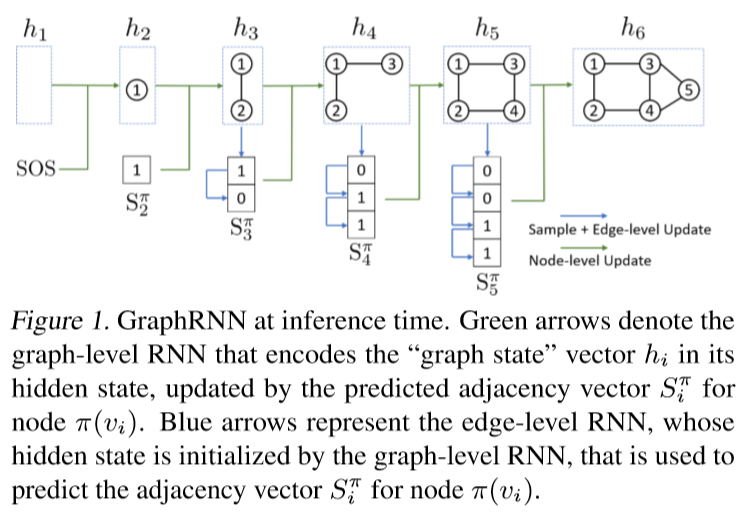
\includegraphics[width=.8\textwidth]{pics/GrpahRNN.png}
    \caption{GraphRNN生成图的过程}
    %\label{fig:my_label}
\end{figure}

GraphRNN模型是基于RNN的模型,以RNN为基础,从一个起始状态,利用RNN逐步生成图的状态,每一步向图中添加一个结点,再利用RNN生成新结点与已存在结点的连接关系,接着再向图中添加结点,重复下去直至EOS。结合之前的定义,$h_i$就是在生成过程中图的状态,它是对已经生成的图的一个encode之后的结果,每步输出$h_i$后就会将$h_i$作为另一个RNN的输入---用于生成边的连接关系的RNN。以上过程就是论文中提到的两个RNN---gaph-level RNN, edge-level RNN。
结合生成图的算法,我们可以知道有这几个部分是比较关键的:$f_{trans}, f_{out}, \mathcal{P}_{\theta_i}$。论文中对这部分都是采用神经网络来实现的,在我理解中$f_{tarns}$就是graph-level 的RNN,被$\theta_i$参数化的$\mathcal{P}_{\theta_i}$({\color{red}论文中没有对其进行详细的说明,$\mathcal{P}_{\theta_i}$具体是什么形式的呢?是全局共用一个$\mathcal{P}_{\theta_i}$吗?})用于生成边的连接关系,即一个二进制序列。
有一个值得注意的点:$S^{\pi}_i$是一个不定长的序列,但是RNN的输入是定长的。论文中是这样处理的这个问题的:采用BFS遍历图,可以得到每个结点的依赖关系,通过对图数据集进行分析,可以得到每个节点依赖的已生成结点的数量$M$的分布,最终在训练时固定下M,即在训练时每个结点所依赖的结点数是确定的,$M$是个超参数。

\par 那么如何进行训练呢?(这部分论文中并没有进行详细的描述,代码中有较详细的过程)\\
首先要将传统格式的图数据转换为论文中定义的序列形式的图。对于每个图,会对其结点进行多次排列,得到多次结点的不同序列,然后根据BFS算法对其进行遍历,可以得到在不同排列下的图生成序列。这样一个图的概率$p(G)$就可以通过求联合分布的边缘分布得到了。其次,在训练的过程中,使用了Teacher Forcing的技术进行训练。


\par 看看这篇论文是否解决了一开始所提到的几个难点呢?
\begin{itemize}
    \item 生成空间太大且可变。个人理解论文中的graph-level和edge-level 的RNN相当于对图进行了编码,能否看作是对整个图的嵌入呢?
    \item 使用序列来表示图的生成过程,将一个确定的图的概率表示为联合概率$p(G, S^{\pi})$的边缘分布。
    \item 复杂的依赖关系。使用BFS遍历图,得到数据集中每个结点所依赖的结点的数量的分布,固定下来作为超参数。(\textbf{{\color{red}这是否可以作为一个改进的点呢?}})
\end{itemize}

\par 未来工作的方向。生成更大规模的图,高效地生成指定条件的图。

其他参考资料:
\begin{enumerate}
    \item \href{https://machinelearningmastery.com/teacher-forcing-for-recurrent-neural-networks/}{What's teacher forcing fir Recurrent Neural Networks?}
\end{enumerate}
